\documentclass[conference]{IEEEtran}
\IEEEoverridecommandlockouts
% The preceding line is only needed to identify funding in the first footnote. If that is unneeded, please comment it out.
\usepackage{cite}
\usepackage{amsmath,amssymb,amsfonts}
\usepackage{algorithmic}
\usepackage{graphicx}
\usepackage{textcomp}
\usepackage{xcolor}
\def\BibTeX{{\rm B\kern-.05em{\sc i\kern-.025em b}\kern-.08em
    T\kern-.1667em\lower.7ex\hbox{E}\kern-.125emX}}

\usepackage{pgfplots}
\usepackage[stdout=false]{pythontex}
% matplotlib2tikz prints messages to stdout, so don't include
% stdout automatically; could also redirect stdout to avoid this
\setpythontexworkingdir{.}
% set PythonTeX to use the document root directory as the working
% directory, so that all plots will be saved there; could use 
% another location, but then would need to specify a path when
% using \input and \InputIfFileExists
    

\usepackage[utf8]{inputenc}
\usepackage[T1]{fontenc}
\usepackage[croatian]{babel}
\begin{document}

\title{Detekcija pakiranih datoteka\\
\thanks{Identify applicable funding agency here. If none, delete this.}
}
\author{\IEEEauthorblockN{Roko Kokan, Jurica Miletić, Ante Sosa}
\IEEEauthorblockA{\textit{Prirodoslovno Matematički fakultet} \\
Zagreb, Hrvatska\\
}
}

\maketitle

\begin{abstract}
Cilj ovog rada je opisati kako detektirati pakirane datoteke uz pomoć alata baziranih na strojnom učenju. Zadatak je osmislila firma ReversingLabs, koja se sama bavi detekcijom malicioznih datoteka. Također, navedena firma nam je dala podatke za treniranje i testiranje našeg modela.
\end{abstract}



\section{Uvod}
Pakiranje je metoda izmjene izvršnih datoteka bez mijenjanja njihove izvorne funkcionalnosti,
ali na način da se datoteka zaštiti od reverznog inženjeringa, da se smanji veličina originalne
izvršne datoteke, ili da se obfuscira maliciozni izvršni kod. Pakiranje podrazumijeva izmjenu
sadržaja datoteke te dodavanje instrukcija koje će prilikom izvršavanja taj sadržaj obnoviti.

Packeri 
modificiraju originalnu izvršnu datoteku na razne načine:
\begin{itemize}
\item Kompresijom podataka
\item Enkripcijom podataka
\item Obfuskacijom
\item Dodavanjem detekcije izvršavanja unutar debuggera ili virtualnog računala
\item Modificiranjem raznih dijelova formata izvršne datoteke
\end{itemize}

U području računalne sigurnosti posebno su učestali packeri za Windows Portable Executable tj. PE datoteke.
PE datoteke su povijesno najčešći nositelji malicioznog koda u 
obliku virusa, ransomwarea, trojanskih konja, itd., te se packeri koriste da bi se taj maliciozni kod prikrio. Klasična statička analiza 
(bez pokretanja datoteka) koju provode antivirusi bazira se na potpisima.
Oni nastaju tako da se prikupe primjeri nekog malwarea te se pronađe niz byteova specifičan za taj malware, 
koji se zatim traži prilikom skeniranja datoteka antivirusom.

\section{Općenito o packerima}

\section{Podaci}
Skup podataka bazirat će se na skupu raznovrsnih packera 
i dodatnim nepakiranim datotekama. Svaki primjer se sastoji 
od dva dijela: originalne datoteke i TitaniumCore izvještaja 
za tu datoteku. 
Cilj zadatka je odvojiti samo pakirane datoteke od 
nepakiranih i raspakiranih, ali će sudionici za razvoj 
modela dobiti detaljnije informacije, poput generalnih 
vrsta packera. U podacima mogu biti varijante višestruko 
pakiranih datoteka, poput dvostruko pakirane datoteke 
koja se tijekom TitaniumCore procesiranja zatim 
jednom raspakira (i dalje se označava kao pakirana).

\section{Problem}


\section{Pristup problemu}
Naš pristup problemu bazirao se na pronalaženju glavnih značajki iz TitaniumCore izvještaja.
Značajke koje smo izvukli iz TitaniumCore izvještaja:
\begin{itemize}
\item  ime odjeljaka
\item	ime importova
\item 	imena apija koji se pozivaju
\item	upozorenja
\item 	imena resursa
\item	veličina filea
\item	veličina odjeljaka 
\item	entropija datoteke
\item 	srednja entropija sekcija
\item	maksimalna entropija sekcija
\item 	minimalna entropija sekcija
\item	vrijeme
\item	veličina opcijskog zaglavlja
\end{itemize}
Nakon toga smo odlučili analizirati dane značajke izgradnjom modela Random Forest Classifiera i XGBoost treniranjem te bi usporedbom važnosti značajki u jednom od modela zadržali one koje su najviše utjecali na rezultat treniranja danog modela.
\section{Realizacija rješenja}
Prvo smo odlučili istrenirati model XGBoost Classifiera iz biblioteke xgboost u pythonu. Da bismo odredili hiperparametre modela koristili smo Randomized Search CV iz biblioteke sklearn (modul model\_selection) kako bismo pretražili prostor vrijednosti za parametre
\begin{itemize} 
\item max\_depth ( $[1, 2,..., 100]$ )
\item min\_child\_weight ( $[0.1, 0.2,..., 3.0]$ )
\item learning\_rate ( $[0.1, 0.2,..., 3.0]$ )
\item base\_score. ( $[0.5, 0.6, 0.7, 0.8, 0.9] $ )
\end{itemize}
% slika ode kako je prošlo traženje
Nakon toga odabiremo parametre koji daju najbolji rezultat (po srednjoj vrijednosti deseterostruke cross validacije koju provede Randomized Search CV) na nasem skupu podataka za pretraživanje. Također, uz zadane parametre za model xgboosta smo odlučili koristiti 100 stabala (po defaultnim postavkama u XGBClassifieru).
% primjer fitanog modela i njegovog procesa treniranja.
Nakon toga smo odlučili istrenirati model Random Forest Classifier, također određujući hiperparametre modela koristeći Randomized Search CV. Željeli smo pretražiti prostor vrijednosti za parametre 
\begin{itemize} 
\item max\_depth ( $[1, 2,..., 100]$ )
\item criterion ( $[True, False]$ )
\item oob\_score ( $[True, False]$ )
\item max\_features ( $[0.001, 0.002,..., 1.000] $ )
\end{itemize}
% slika ode kako je prošlo traženje
Nakon toga odabiremo parametre na isti način kao i kod XGBClassifiera. Također koristit ćemo 100 stabala (po defaultnim postavkama).
% primjer fitanog modela i njegovog procesa treniranja.
S obzirom na prikazano, XGBoost model nakon treniranja na podacima daje bolje rezultate, te ćemo njega koristiti za daljnju analizu značajki.

\begin{figure}[h]
\centering
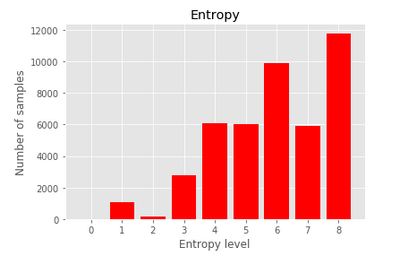
\includegraphics{ent.png}
\end{figure}

\section*{Acknowledgment}

The preferred spelling of the word ``acknowledgment'' in America is without 
an ``e'' after the ``g''. Avoid the stilted expression ``one of us (R. B. 
G.) thanks $\ldots$''. Instead, try ``R. B. G. thanks$\ldots$''. Put sponsor 
acknowledgments in the unnumbered footnote on the first page.

\section*{References}

Please number citations consecutively within brackets \cite{b1}. The 
sentence punctuation follows the bracket \cite{b2}. Refer simply to the reference 
number, as in \cite{b3}---do not use ``Ref. \cite{b3}'' or ``reference \cite{b3}'' except at 
the beginning of a sentence: ``Reference \cite{b3} was the first $\ldots$''

Number footnotes separately in superscripts. Place the actual footnote at 
the bottom of the column in which it was cited. Do not put footnotes in the 
abstract or reference list. Use letters for table footnotes.

Unless there are six authors or more give all authors' names; do not use 
``et al.''. Papers that have not been published, even if they have been 
submitted for publication, should be cited as ``unpublished'' \cite{b4}. Papers 
that have been accepted for publication should be cited as ``in press'' \cite{b5}. 
Capitalize only the first word in a paper title, except for proper nouns and 
element symbols.

For papers published in translation journals, please give the English 
citation first, followed by the original foreign-language citation \cite{b6}.

\begin{thebibliography}{00}
\bibitem{b1} G. Eason, B. Noble, and I. N. Sneddon, ``On certain integrals of Lipschitz-Hankel type involving products of Bessel functions,'' Phil. Trans. Roy. Soc. London, vol. A247, pp. 529--551, April 1955.
\bibitem{b2} J. Clerk Maxwell, A Treatise on Electricity and Magnetism, 3rd ed., vol. 2. Oxford: Clarendon, 1892, pp.68--73.
\bibitem{b3} I. S. Jacobs and C. P. Bean, ``Fine particles, thin films and exchange anisotropy,'' in Magnetism, vol. III, G. T. Rado and H. Suhl, Eds. New York: Academic, 1963, pp. 271--350.
\bibitem{b4} K. Elissa, ``Title of paper if known,'' unpublished.
\bibitem{b5} R. Nicole, ``Title of paper with only first word capitalized,'' J. Name Stand. Abbrev., in press.
\bibitem{b6} Y. Yorozu, M. Hirano, K. Oka, and Y. Tagawa, ``Electron spectroscopy studies on magneto-optical media and plastic substrate interface,'' IEEE Transl. J. Magn. Japan, vol. 2, pp. 740--741, August 1987 [Digests 9th Annual Conf. Magnetics Japan, p. 301, 1982].
\bibitem{b7} M. Young, The Technical Writer's Handbook. Mill Valley, CA: University Science, 1989.
\end{thebibliography}
\vspace{12pt}
\color{red}
IEEE conference templates contain guidance text for composing and formatting conference papers. Please ensure that all template text is removed from your conference paper prior to submission to the conference. Failure to remove the template text from your paper may result in your paper not being published.

\end{document}
